\documentclass[12pt, c]{beamer}
% Setup appearance:

% Standard packages
\usepackage[french]{babel}
\usepackage{times}
\usepackage[T1]{fontenc}
\usepackage{float}
\usepackage{multirow}
\usepackage{subfigure}
\usepackage{pifont}
\usepackage{tikz}
\usepackage{morewrites}
\usepackage{amsmath}
%\usepackage{subfig}
\usetikzlibrary{arrows}
\tikzstyle{block}=[draw opacity=0.7,line width=1.4cm]
\DeclareOption{english}{\trans@use@and@alias{english}{English}}
\ProcessOptions*

\mode<presentation> {
	\definecolor{bgcol}{RGB}{255,255,255}
	\definecolor{grencol}{RGB}{0,102,0}
	\definecolor{rulecol}{RGB}{3,16,67}
	\definecolor{boxtitre}{RGB}{37,45,137}
	}

  \usetheme{Warsaw}
	%\usecolortheme[named=rulecol]{structure}
	\usefonttheme[onlysmall]{structurebold}
	\usefonttheme{structureitalicserif}
	\useinnertheme{rounded}
	\useoutertheme{split}
	
	\beamertemplateshadingbackground{bgcol}{bgcol} % pour jouer sur la couleur % du fond
	\beamertemplatetransparentcovereddynamic
	\setbeamertemplate{background canvas}[vertical shading][top=white, bottom=white!60!white]
	%\setbeamercolor{normal text}{bg=rulecol,fg=black}
	%\setbeamercolor{title in head}{bg=rulecol!80,fg=bgcol}
	\setbeamercolor{title in foot}{bg=black,fg=white}
	\setbeamercolor{author in head}{bg=rulecol,fg=bgcol}
	\setbeamercolor{author in foot}{bg=black!80,fg=white}
	\setbeamercolor{section in head}{bg=black,fg=bgcol}
	\setbeamercolor{section in foot}{bg=rulecol!80,fg= bgcol}
	\setbeamercolor{subsection in head}{bg=black,fg=bgcol}
	\setbeamercolor{subsection in foot}{bg=rulecol,fg=bgcol}
	\setbeamercolor{logo}{bg=rulecol,fg=white}
	\setbeamercolor{section in head/foot}{bg=black!90,fg=white}
	\setbeamercolor{subsection in head/foot}{bg=rulecol!90,fg=white}
	\setbeamercolor{boiterouge}{bg=red!60,fg=black}
	\setbeamercolor{boiterougeB}{bg=red,fg=black}
	\setbeamercolor{boiteblanche}{bg=white,fg=black}
	\setbeamercolor{boiteverte}{bg=green,fg=black}
	\setbeamercolor{boiteblue}{bg=rulecol,fg=white}
	
	\setbeamerfont*{frametitle}{size=\normalsize}
	
	
  \setbeamertemplate{navigation symbols}{}
	\setbeamertemplate{itemize item}[square]
	\setbeamertemplate{enumerate item}[ball]
	\setbeamertemplate{itemize subitem}[triangle]
	\setbeamertemplate{itemize subsubitem}[circle]
	\logo{
\includegraphics[height=5mm]{images/logouniv.png}}
	\setbeamertemplate{footline}{
		\leavevmode%
		\hbox{\hspace*{-0.06cm}
		
		\begin{beamercolorbox}[wd=.265\paperwidth,ht=2.25ex,dp=1ex,left]{author in foot}%
			\usebeamerfont{author in head/foot}\insertshortauthor%~~(\insertshortinstitute)
		\end{beamercolorbox}%
		
		\begin{beamercolorbox}[wd=.6\paperwidth,ht=2.25ex,dp=1ex,center]{title in foot}%
			\usebeamerfont{title in head/foot}\insertshorttitle
		\end{beamercolorbox}%
		
		\begin{beamercolorbox}[wd=.135\paperwidth,ht=2.25ex,dp=1ex,right]{section in foot}%
			\usebeamerfont{logo}\textcolor[rgb]{1,0.41,0.13}{\insertshortdate{}}\hspace*{0.4em}
			\insertframenumber{} / \inserttotalframenumber
		\end{beamercolorbox}}%
		
		\vskip0pt%
	}
\renewcommand{\raggedright}{\leftskip=0pt \rightskip=0pt plus 0cm}

\title[Storage Virtualization]{}

\author[$\;\;$ TCHIO AMOUGOU Styves Daudet]{}

\date[Janvier 2021]{janvier 2021}

%\subject{Mémoire de Master 2}
\begin{document}
\begin{frame}
\transfade
	\vspace{-0.3cm}
	\begin{figure}
		\begin{center}
		
\includegraphics[width=11cm,height=1.2cm]{images/enteteUds.PNG}
		\end{center}
	\end{figure}
	
	\begin{center}
	\tiny{\textsc{\textcolor{black}{DSCHANG SCHOOL OF SCIENCES AND TECHNOLOGY}}}\\
		\tiny{Unité de Recherche en Informatique Fondamentale, Ingénierie et  Application (URIFIA)}
	\end{center}
	\vspace{0.05cm}
\fcolorbox{boxtitre}{boxtitre}{\parbox{1\linewidth}{

\vspace{-0.3cm}
\begin{center}

\vspace{0.05cm}
 \textcolor{bgcol}{Storage Virtualization}

%\vspace{0.1cm}
\end{center}

\vspace{-0.1cm}
}}
\begin{center}
\fcolorbox{bgcol}{bgcol}{
\parbox{1\linewidth}{
\begin{center}
\vspace{-0.5cm}
\footnotesize Présenté par :\\ \textbf{\textcolor{boxtitre}{ TCHIO AMOUGOU Styves daudet}} \\
\scriptsize{\textit{Matricule : CM-UDS-14SCI0251}}\\
 \tiny{\textit{Licencié en Informatique Fondamentale}}\\
 \vspace{0.3cm}
				\scriptsize{\textit{Sous la direction de }}\\
				\scriptsize{\textbf{Dr BOMGNI ALAIN Bertrand} }\\
								\tiny{(\textit{Chargé de Cours, Université de Dschang})}\\
				\end{center}
}}
\end{center}
\end{frame}

\begin{frame}{\scriptsize Sommaire}
\transwipe
\scriptsize
  \tableofcontents
\end{frame}

\section{Introduction}

%% definitions de la virtualisation 

	\subsection{Definition}
	\setbeamercovered{invisible}
		\begin{frame}{Définitions}
		\transwipe
	
		\vspace{-0.25cm}
			\begin{block}{}
				 \begin{itemize}
			 		\item 
			 			\begin{flushleft}
			 				\textbf{La virtualisation : } est une technologie qui consiste à
			 				l’abstraction des ressources d’un équipement physique (ordinateur, routeur,
			 				switch, ...) (Carapinha  Jiménez, 2009). 
			 			\end{flushleft}
			 		\item
			 			\begin{flushleft}
			 				\textbf{Une machine Virtuelle : } est un equipement logique crée a partie 
			 				d'un equipement physique et pocedent le meme caracteristiques que ce dernie
			 				(processeur, memoire stokage, Ram,etc ...)
						\end{flushleft}			 			 
			 		\item
			 			\begin{flushleft}
			 				\textbf{L’hyperviseur : } est un logicielle qui  permet de
			 				créer une ou plusieurs machines virtuelles dans les limites de la quantité
			 				de ressources disponibles dans l’équipement physique.
			 				
			 				\begin{flushleft}
			 				Exemple: Xen, Oracle VM, VmWare workstation, virtualBox, Citrix, ...
			 				\end{flushleft}
			 			\end{flushleft}
			 	\end{itemize}
	
			\end{block}	
		\end{frame}
		%% exemple de virtualisation sur une image		
		\begin{frame}{Example}
			\transfade
			\vspace{-0.3cm}
			\begin{figure}
				\begin{center}
					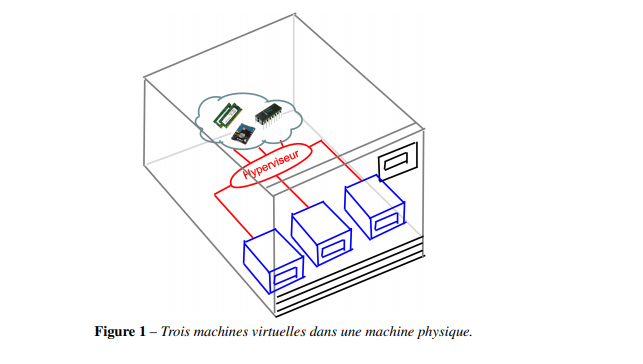
\includegraphics[width=11cm,height=7cm]{images/ex_virtual.PNG}
				\end{center}
			\end{figure}
		\end{frame}
	
	
%% avantage de la virtualisation	
	\subsection{Avantages}
		\setbeamercovered{invisible}
			\begin{frame}{Avantages}
				\transwipe
				\vspace{-0.25cm}
				\begin{block}
					
				\end{block}
			\end{frame}
			

		
		
%% les different  types de virtualisation
		\subsection{Formes de virtualisation}
			\setbeamercovered{invisible}
			\begin{frame}{Formes de virtualisation}
				\transwipe
				\vspace{-0.25cm}
				\begin{block}{}
					\begin{itemize}
						\item
							Virtualisation de memoire
							
						\item
							Virtualisation de reseau
							
						\item
							Virtualisation de serveur
							
						\item
							Virtualisation de stockage
					\end{itemize}
				\end{block}
			\end{frame}
%% sections sur la virtualisation des reseaux 
\begin{frame}
	\transdissolve
	\vspace{1cm}
		\begin{center}
			\huge \textbf{\textsc{Virtualisation des reseaux}}
		\end{center}
	\end{frame}

\section{Virtualisation des reseaux}
	%% defintions
	\subsection{Définitions}
		\begin{frame}{Définitions}
			\transwipe
			\vspace{-0.25cm}
			\begin{block}{}
				\begin{itemize}
					\item 
						\begin{flushleft}
							L’interconnexion des machines virtuelles entre elles constitue un
							\textbf{réseau virtuel} 
						\end{flushleft}
					\item
						\begin{flushleft}
							\textbf{Virtualisation du réseau : } est la reproduction
							logicielle d’un réseau physique. 
						\end{flushleft}
				\end{itemize}
			\end{block}
			\end{frame}
	%% avantages
		\subsection{Avantages}
		\setbeamercovered{invisible}
			\begin{frame}{Virtualisation}
			\transwipe
			\vspace{-0.25cm}
				\begin{block}
	
			\end{block}
			\end{frame}
%% section sur le sdn(softward defined network)
\begin{frame}
	\transdissolve
	\vspace{1cm}
		\begin{center}
			\huge \textbf{\textsc{Réseaux définis par logiciels (SDN)}}
		\end{center}
	\end{frame}

\section{Réseaux définis par logiciels (SDN)}
	%% defintions
	\subsection{Definitions}
		\setbeamercovered{invisible}
			\begin{frame}{definitions}
			\transwipe
			\vspace{-0.25cm}
				\begin{block}
	
			\end{block}
			\end{frame}
	%% avantages
		\subsection{Avantages}
		\setbeamercovered{invisible}
			\begin{frame}{Virtualisation}
			\transwipe
			\vspace{-0.25cm}
				\begin{block}
	
			\end{block}
			\end{frame}
%% section sur la virtualisation des  stockage 
\begin{frame}
	\transdissolve
	\vspace{1cm}
		\begin{center}
			\huge \textbf{\textsc{Virtualisation des stockage}}
		\end{center}
	\end{frame}
\section{Virtualisation des stockage}
	%% definition
	\subsection{Definition}
		\setbeamercovered{invisible}
			\begin{frame}{Definiton}
			\transwipe
			\vspace{-0.25cm}
				\begin{block}
	
			\end{block}
			\end{frame}
			
			
			
	\subsection{Why, What, Where and How?}
		\setbeamercovered{invisible}
			\begin{frame}{Definiton}
			\transwipe
			\vspace{-0.25cm}
				\begin{block}
	
			\end{block}
			\end{frame}
	
	
	
	
	\begin{frame}
	\transdissolve
	\vspace{1cm}
		\begin{center}
			\huge \textbf{\textsc{Merci pour votre aimable attention}}
		\end{center}
	\end{frame}
	
%\bibliographystyle{apacite} 
%\bibliography{References/references}

%\subject{Mémoire de Master 2}
\begin{frame}
\transfade
	\vspace{-0.3cm}
	\begin{figure}
		\begin{center}
		
\includegraphics[width=11cm,height=1.2cm]{images/enteteUds.PNG}
		\end{center}
	\end{figure}
	
	\begin{center}
	\tiny{\textsc{\textcolor{black}{DSCHANG SCHOOL OF SCIENCES AND TECHNOLOGY}}}\\
		\tiny{Unité de Recherche en Informatique Fondamentale, Ingénierie et  Application (URIFIA)}
	\end{center}
	\vspace{0.05cm}
\fcolorbox{boxtitre}{boxtitre}{\parbox{1\linewidth}{

\vspace{-0.3cm}
\begin{center}

\vspace{0.05cm}
 \textcolor{bgcol}{Storage Virtualization}

%\vspace{0.1cm}
\end{center}

\vspace{-0.1cm}
}}
\begin{center}
\fcolorbox{bgcol}{bgcol}{
\parbox{1\linewidth}{
\begin{center}
\vspace{-0.5cm}
\footnotesize Présenté par :\\ \textbf{\textcolor{boxtitre}{ TCHIO AMOUGOU Styves daudet}} \\
\scriptsize{\textit{Matricule : CM-UDS-14SCI0251}}\\
 \tiny{\textit{Licencié en Informatique Fondamentale}}\\
 \vspace{0.3cm}
				\scriptsize{\textit{Sous la direction de }}\\
				\scriptsize{\textbf{Dr BOMGNI ALAIN Bertrand} }\\
								\tiny{(\textit{Chargé de Cours, Université de Dschang})}\\
				\end{center}
}}
\end{center}
\end{frame}
\end{document}